\section{Analyse der vorhandenen Implementierung}
Zur Verfügung steht eine Java- sowie eine C-Implementierung des Algorithmus. Die Implementierung in C wurde näher betrachtet, da diese die Möglichkeit bietet, Algorithmusschritte mithilfe der Grafikkarte zu beschleunigen.

\subsection{Aufbau des Programmes}
Das Programm lässt sich mit einer JSON-Konfigurationsdatei, welche im ersten Schritt eingelesen und deserialisiert wird, parametrisieren. Hier werden beispielsweise Algorithmushyperparameter wie $\tau$ und $\epsilon$ bestimmt oder die Berechnung über die Grafikkarte aktiviert bzw. deaktiviert.\\
Der Datensatz wird als CSV-Datei bereitgestellt, welche in einen Vektor mit Elementen einer internen Datenstruktur „DataPoint“ umgewandelt wird. DataPoint ist hier irreführend, da die Datenstruktur eine Dimension und die Werte dieser Dimension aller Datensätze hält.\\
Mit Nutzung des Strategy-Patterns wird abhängig der Konfiguration die sequenzielle oder die parallele Subscale Strategie geladen.\\
Die Methode „calculateClusterCandidates“, die beide Strategien zur Verfügung stellen, durchläuft den eingangs beschriebenen Algorithmus und liefert die Subspaces des übergebenen Datensatzes. Aus den Subspaces werden im Anschluss Cluster mittels DBSCAN ermittelt. Die gefundenen Cluster werden in einer CSV-Datei persistiert.

\subsection{Sequenzielle Implementierung}
Die sequenzielle Strategie instanziiert factory-ähnlich Abarbeitungsklassen, welche als Referenz an die generische Methode „calculateAllSlices“ übergeben werden.\\
Die Methode unterteilt den Gesamtraum in disjunkte Teilräume. Für jeden Teilraum werden sequenziell die Dense Units bestimmt, gefiltert und zu Subspaces geclustert um diese Zwischenergebnisse anschließend pro Slice in einer eigenen CSV-Datei abspeichern zu können.\\
Im Anschluss werden die Dateien mit Zwischenergebnissen Datei für Datei zu einem Endergebnis kombiniert. Das Gesamtergebnis wird dem DBSCAN-Algorithmus übergeben. Die finalen Cluster werden in eine Datei geschrieben.

\subsection{GPU-beschleunigte Implementierung}
Die GPU beschleunigte Implementierung unterscheidet sich von der sequenziellen Implementierung bei der Instanziierung der Abarbeitungsklassen. „DenseUnitCreator“ und „SubspaceJoiner“ ersetzen die CPU basierten Berechnungen durch Berechnungen auf der Grafikkarte.\\
Das Zusammenführe der Teilergebnisse erfolgt mit der identischen Logik wie im sequenziellen Algorithmus.

\section{Restrukturierung in einer neuen Anwendung}
Mit einer architektonischen Umstrukturierung sollen verschiedene Phasen des Algorithmus beliebig austauschbar werden, sodass verschiedene Verteil- und Beschleunigungsverfahren miteinander verglichen werden können.\\
Subscale lässt sich in die Phasen Import, CoreSet-Seeker, DenseUnit-Generation, Subspace-Detection, Subspace-Combination und Export unterteilen. Jede der Phasen wird mit einem Interface abstrahiert. Für ein Proof of Conecpt soll der Subscale Algorithmus in einer sequenziellen Ausführung mit der Neustrukturierung implementiert werden.

\subsection{Import}
Die Importer implementieren eine Methode, die Tensordaten aus einem Medium auslesen und diese als Kollektion der Datenstruktur „Dimension“ bereitstellen. Die Dimension hält ihre Größe, sowie ein Set von Punkten.
\begin{figure}[h]
	\centering
	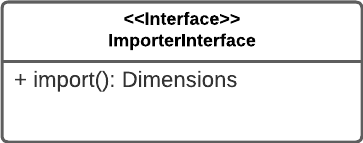
\includegraphics[width=0.5\textwidth]{./Bilder/Restrukturierung/Importer.png}
	\caption{ImporterInterface}
\end{figure}
Für das Projekt konkret implementiert wurde ein CsvImporter, welcher die Daten aus einer CSV-Datei ausließt und in Dimensions zur weiteren Verarbeitung umwandelt.\\
Der Datenimport kann hier mit weiteren konkreten Implementierungen beliebig ergänzt oder ersetzt werden. Denkbar wäre beispielsweise der Import anderer Datenformate wie JSON oder XML oder das Lesen von entfernt bereitgestellten Ressource wie beispielsweise eine CSV-Datei auf einem SFTP-Server.

\subsection{CoreSet-Seeker}
Der CoreSet-Seeker iteriert durch die übergebene Dimension und liefert für diese alle gefundenen CoreSets.
\begin{figure}[h]
	\centering
	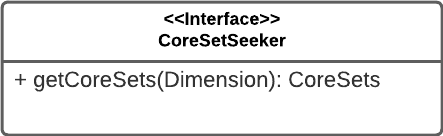
\includegraphics[width=0.5\textwidth]{./Bilder/Restrukturierung/CoreSetSeeker.png}
	\caption{CoreSetSeekerInterface}
\end{figure}
Konkret implementiert wurde ein SequentialCoreSetGenerator. Dieser iteriert mit zwei geschachtelten for-Schleifen über alle Punkte der übergebenen Dimension und berechnet hiermit die euklidische Distanz zwischen allen Punkten. Unterschreitet diese $\epsilon$, werden die Punkte zu einem CoreSet zusammengefasst.\\
Weiter denkbar wäre die Implementierungen ParallelCoreSetGenerator, welcher die CoreSets auf einer GPU berechnen lässt, indem mehreren Threads unterschiedliche Dimensionen oder gar einzelne Punkte einer Dimension zugewiesen werden. Die Resultate werden im Anschluss gesammelt und zusammengeführt.\\
Auch eine Implementierung DistributeCoreSetGenerator könnte den Algorithmus beschleunigen. Diese Implementierung dekoriert eine der vorherigen Implementierungen, indem diese den Aufruf mittels GRPC an entfernte Maschinen weiterleitet, auf dessen Berechnungsergebnisse wartet um diese dann zusammengeführt zurückgeben zu können.

\subsection{Dense Unit Generator}
Der Dense Unit Generator erstellt für jedes CoreSet alle Kombinationen der Größe $\tau$. Diese Kombinationen werden in der Datenstruktur DenseUnit abgelegt. DenseUnits werden gesammelt und als Collection zurückgegeben.
\begin{figure}[h]
	\centering
	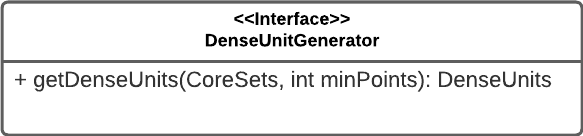
\includegraphics[width=0.5\textwidth]{./Bilder/Restrukturierung/DenseUnitGenerator.png}
	\caption{DenseUnitGeneratorInterface}
\end{figure}
Die Implementierung SequentialDenseUnitGenerator übernimmt genau dies in for-Schleifen. Zukünftige Implementierungen ParallelDenseUnitGenerator und DistributedDenseUnitGenerator parallelisieren die Generierung der Dense Units zum Beispiel durch Zuweisung eines CoreSets pro Thread und verteilen diese.

\subsection{Subspace Detector}
Der Subspace Detector untersucht Dense Units auf Kollisionen und findet dadurch Subspaces: Anhäufungen vom Punkten über mehrere Dimensionen.
\begin{figure}[h]
	\centering
	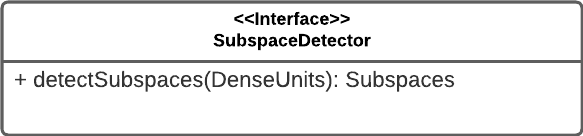
\includegraphics[width=0.5\textwidth]{./Bilder/Restrukturierung/SubspaceDetector.png}
	\caption{SubspaceDetectorInterface}
\end{figure}
Der SequentialSubspaceDetector iteriert über alle DenseUnits und prüft deren Signatur auf Kollision mit anderen DenseUnits. Kollidieren mehrere Dense Units, bilden diese einen Subspace. Die Methode gibt alle entdeckten Subspaces zurück.\\
Ein ParallelSubspaceDetector und ein DistributedSubspaceDetector könnten die gleiche Aufgabe durch Verteilen der zu untersuchenden DenseUnits auf Threads und durch Verteilen auf entfernte Maschinen und anschließendes Zusammenführen erledigen.

\subsection{Subspace Combiner}
Der Subspace Combiner erstellt aus den Subspaces, welche mehrere Dense Units bündeln, Cluster.
\begin{figure}[h]
	\centering
	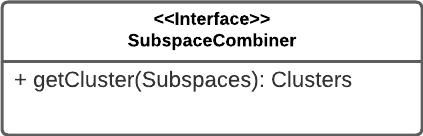
\includegraphics[width=0.5\textwidth]{./Bilder/Restrukturierung/SubspaceCombiner.png}
	\caption{SubspaceCombinerInterface}
\end{figure}
Der SequentialSubspaceCombiner iteriert über alle Punkte der im Subspace vorkommenden Dense Units und eliminiert Duplikate beim Zusammenfassen zu Cluster. Dies geschieht durch Iteration über alle Subspaces, deren Dense Units und den dort enthaltenen Punkten.\\
Der Bau der Cluster funktioniert für jeden Subspace unabhängig, weswegen die Subspacekombination in einem ParallelSubspaceCombiner und einem DistributedSubspaceCombiner parallelisiert und verteilt werden kann.

\subsection{Factory}
Die Definition der Schnittstellen erlaubt eine beliebige Konfiguration des Algorithmus. Eine Subscale Klasse wird mit der Übergabe eines CoreSetSeekers, eines DenseUnitGenerators, eines SubspaceDetectors und eines SubspaceCombiners instanziiert. Deren Methode „getClusters“ nimmt ein Set von Dimensionen, iteriert über diese um mit dem CoreSetSeeker alle CoreSets zu erhalten, bildet aus den CoreSets Dense Units, in welchen anschließend Subspaces gesucht werden, die die Methode schlussendlich zu Cluster kombiniert. DBSCAN übernimmt das finale Clustering der durch Subscale gefundenen Clusterkandidaten.
\begin{figure}[h]
	\centering
	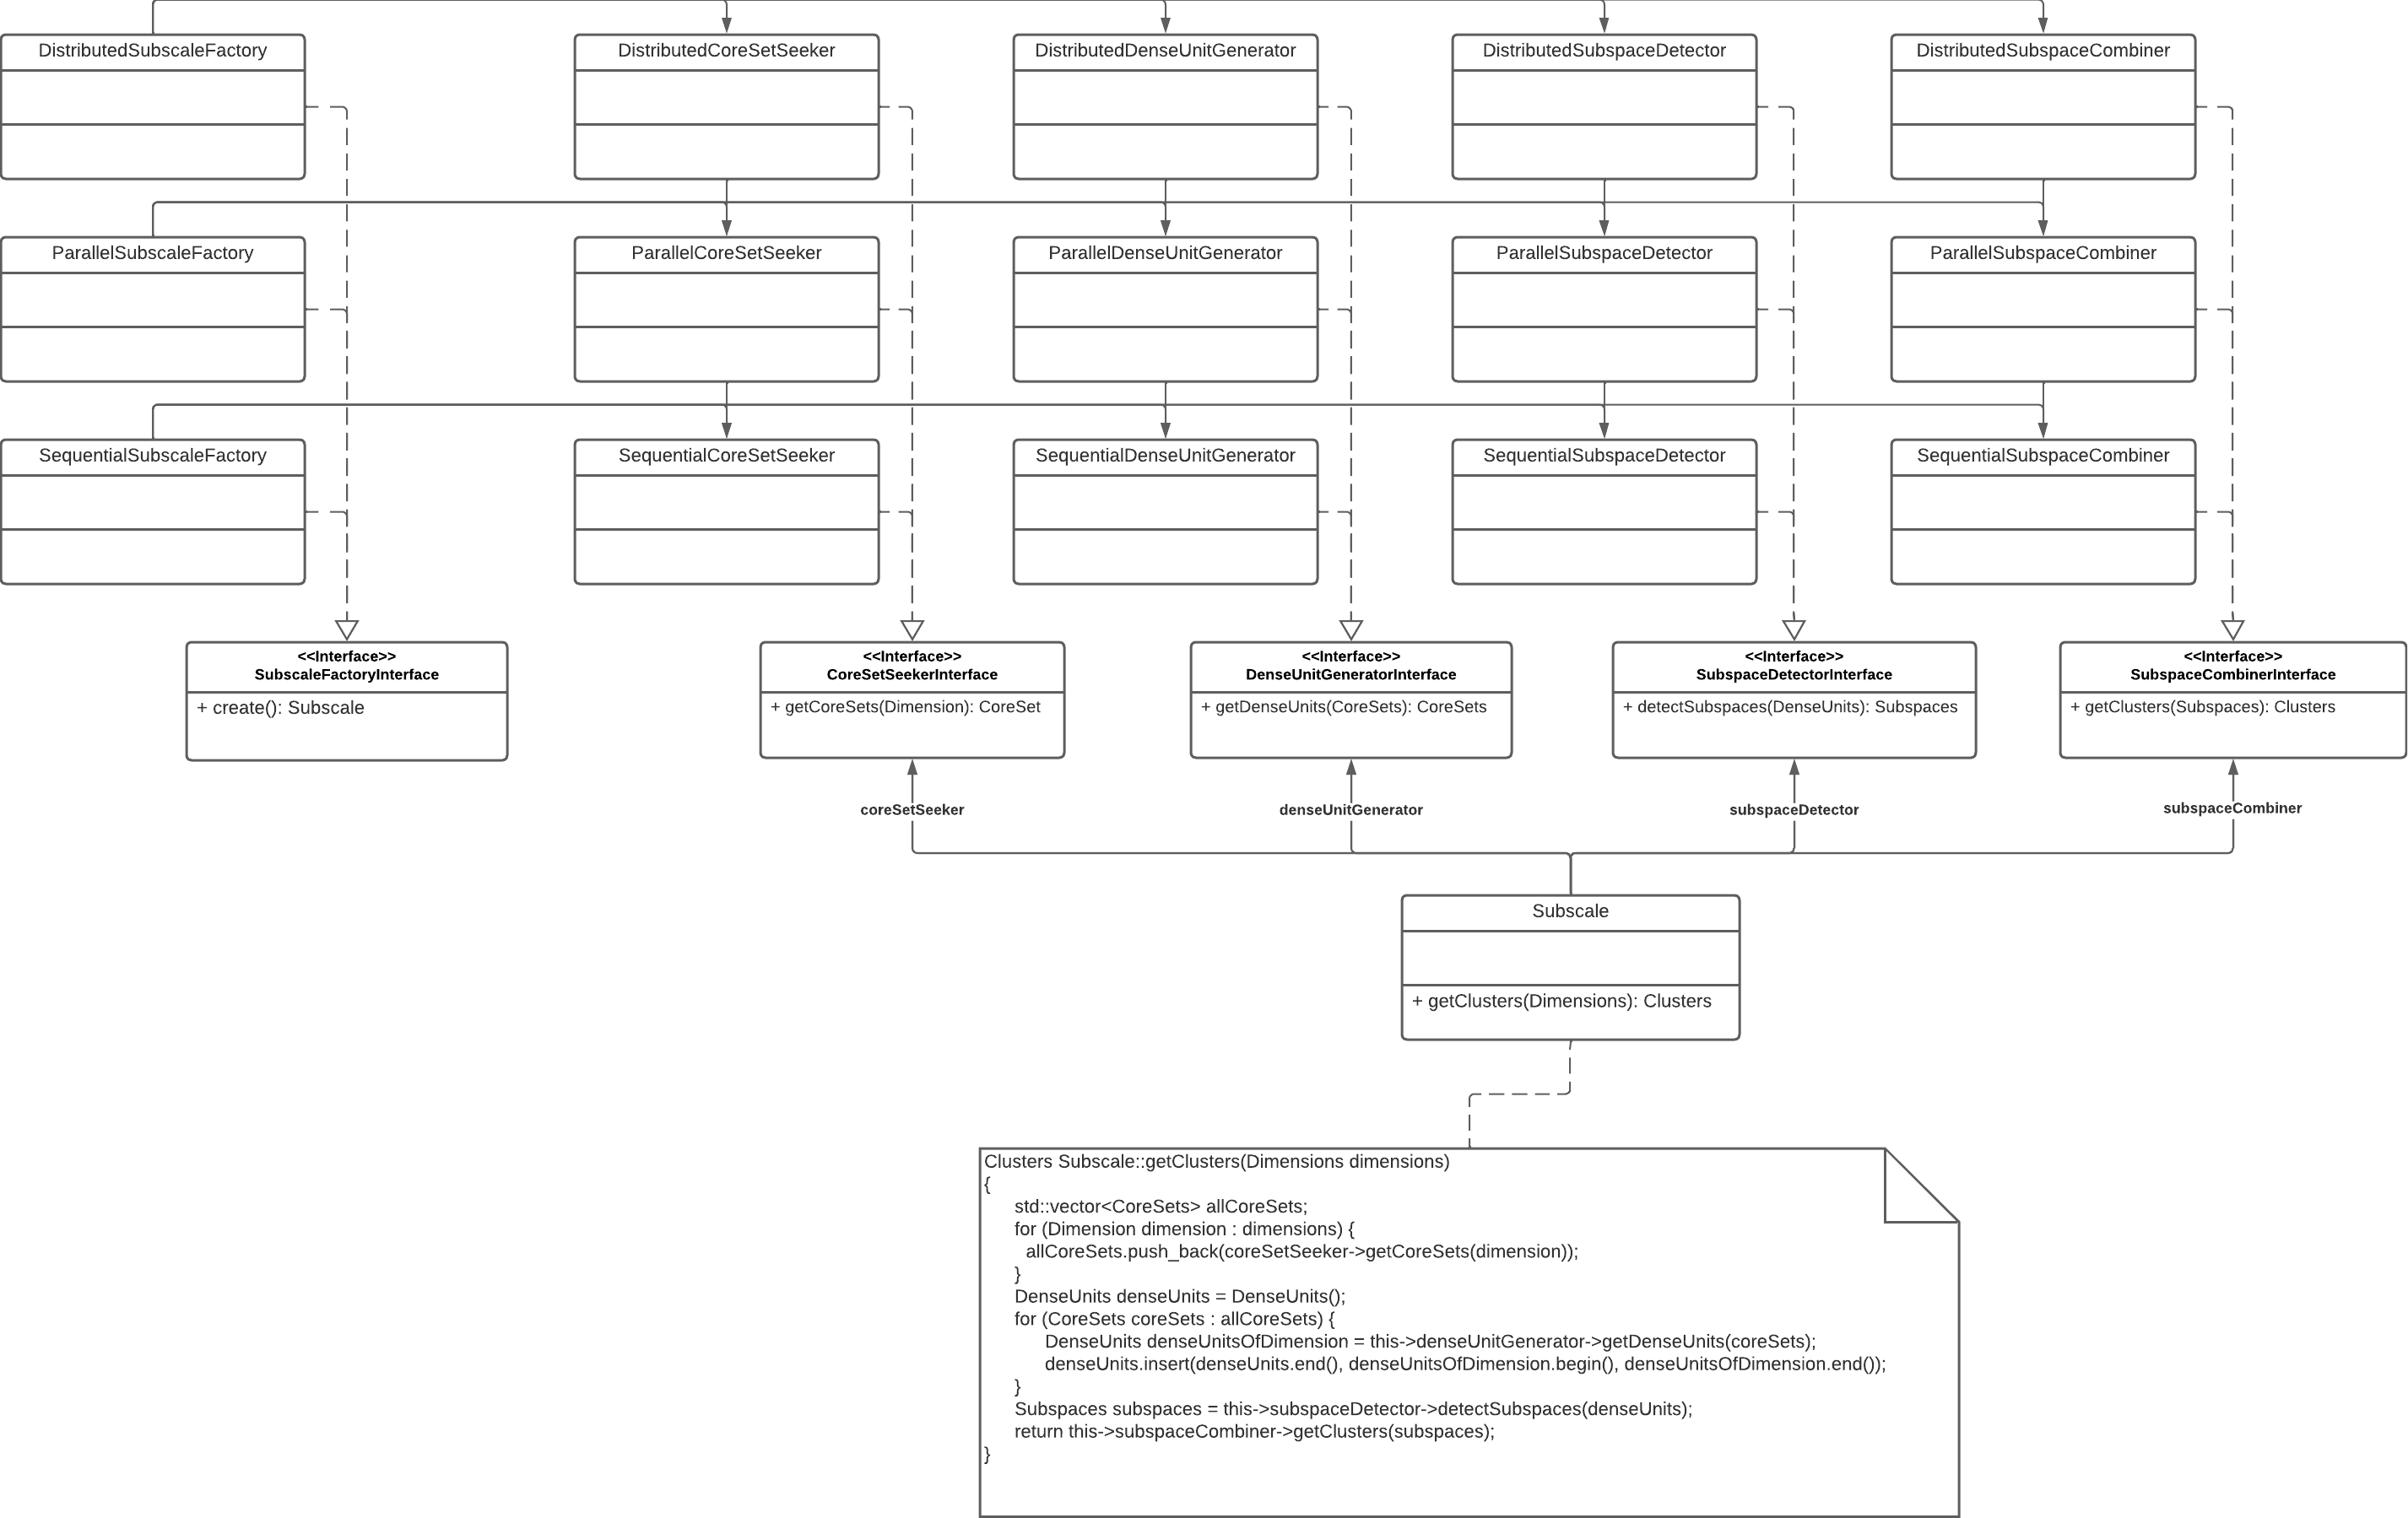
\includegraphics[width=0.9\textwidth]{./Bilder/Restrukturierung/Factory.png}
	\caption{Factory}
\end{figure}
Da diese Architektur dem Open-Close-Principle folgt, bietet sie die Möglichkeit, dass mehrere Entwickler zeitgleich und konfliktfrei verschiedene Module entwickeln können. Außerdem erlaubt sie eine feingranulare Analyse über Optimierungsoptionen. So kann der Algorithmus beispielsweise aus einen verteilten CoreSetSeeker, einem parallelen DenseUnitGenerator, einem sequenziellen SubspaceDetector und einem parallelen SubspaceCombiner bestehen. Für beliebige Kombinationen kann die Ausführungszeit gemessen werden, um zu analysieren, bei welchen Prozessschritten durch die Parallelisierung und Verteilung tatsächlich ein Zeitgewinn zu verzeichnen ist.

\subsection{Probleme}
Da parallel die Anpassung der Codevorlage analysiert wurde, entschieden wir uns für ein „Proof of Concept“. Nach dessen Umsetzung wollen wir abwägen, welche Lösung für die Projektumsetzung herangezogen wird.\\
Das Proof of Concept umfasste die dargelegte Architektur und die konkrete Implementierung für die sequenzielle Abarbeitung des Algorithmus. Der SequentialCoreSetSeeker, der SequentialDenseUnitGenerator, der SequentialSubspaceDetector und der SequentialSubspaceCombiner wurden implementiert und in einer SequentialSubscaleFactory kombiniert. Ebenfalls implementiert wurde ein CSV-Importer zum Einlesen des Testdatensatzen.\\
Für kleine Datensätze war die Umsetzung lauffähig und lieferte Ergebnisse. Allerdings war die Laufzeit um ein Vielfaches länger. Größere Datensätze konnten aufgrund eines Speicherüberlaufs nicht bearbeitet werden. Bei der Implementierung wurde das von C++ benötigte akribische Speichermanagement zu sehr vernachlässigt was die Performanz der Anwendung massiv einschränkte.\\
Des Weiteren entschieden wir uns nach der PoC-Phase gegen die Fortsetzung dieser Lösung, da die Cuda-Codeabschnitte aus der Codevorlage nicht einfach übernommen werden konnten. Für Anpassungen im Cuda-Code fehlt im Team die Expertise. Eine parallele Umsetzung ist folglich nicht möglich.